\documentclass[12pt]{article}

%opening
\title{Tesina Segnali e Sistemi 2022}
\author{Lorenzo Franceschetti Mat. 2000263}
\date{}
\usepackage[margin=2cm]{geometry}
\usepackage{graphicx}
\usepackage{float}
\begin{document}

\maketitle

\section{Introduzione}

È dato il segnale $x_{t}(t)$, ottenuto dalla modulazione in ampiezza del segnale $x(t)$ alla frequenza $F_{m}$: 
\begin{equation}
	x_{t}(t) = x(t) cos(2\pi F_{m}t)
\end{equation} 
Chiamata con $X_{t}(f)$ la trasformata del segnale $x_{t}(t)$, si ha che: 
\begin{equation}
	X_{t}(f) = \frac{1}{2}[X(f - F_{m}) + X(f + F_{m})]
\end{equation}
dove $X(f)$ rappresenta la trasformata del segnale $x(t)$. Dallo studio in frequenza del segnale dato ci si attende quindi di trovare due gruppi di frequenze (corrispondenti a $X(f)$) centrati in $f = F_{m}$ e in $f = -F_{m}$. Una volta individuata la frequenza di modulazione, per recuperare il segnale $x(t)$ si può procedere come segue: 
\begin{itemize}
	\item Si moltiplica il segnale modulato per $2cos(2\pi F_{m}t)$
	\item Si filtra il segnale ottenuto tramite un filtro con risposta in frequenza data da
	\begin{equation}
		H_{lp}(f) = rect \biggl(\frac{f}{2B_{x}}\biggr)
	\end{equation}
	dove $B_{x}$ è la larghezza di banda monolatera del segnale $x(t)$
\end{itemize}

\section{Studio del segnale modulato}

Il segnale $x_{t}(t)$ e la sua trasformata di Fourier $X_{t}(f)$ risultano essere:
\begin{figure}[H]
	\centering
	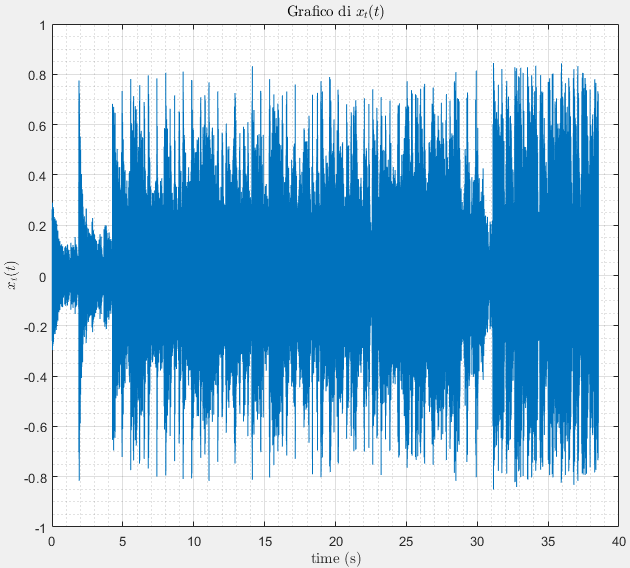
\includegraphics[width=0.45\linewidth]{./images/x_t.png}
	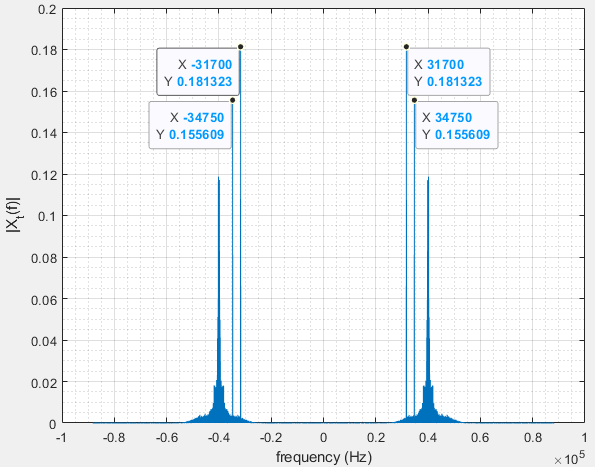
\includegraphics[width=0.45\linewidth]{./images/fft_x_t.png}
\end{figure}

Trascurando per il momento i due picchi a $\pm31700Hz$ e $\pm34750Hz$, il grafico di $|X_{t}(f)|$ mostra due gruppi di componenti, uno per frequenze positive e uno per quelle negative, centrati rispettivamente sugli assi $f = \pm40000Hz$, come atteso per un segnale modulato in ampiezza con un coseno di frequenza $F_{m} = 40000Hz$.

\section{Eliminazione degli artefatti dal segnale}

Il segnale demodulato presenta dei disturbi in $\pm5250Hz$ e $\pm8300Hz$, effetto della demodulazione dei disturbi ad alta frequenza in $\pm31700Hz$ e $\pm34750Hz$ presenti nel segnale originario.

Per ridurre questi disturbi si possono adottare dei notch filter, in grado di attenuare il segnale in un intervallo molto ristretto di frequenze. Tali filtri sono caratterizzati da una frequenza centrale $F_{filter}$ attorno alla quale si sviluppa l'intervallo di attenuazione. Dovendo filtrare due componenti distanti tra loro più dell'ampiezza della banda attenuata del filtro, è necessario impiegare due distinti notch filter, centrati in $F_{filter} = 31700Hz$ e in $F_{filter} = 34750Hz$. All'ascolto si nota come, oltre alla mancanza dei fischi, anche alcuni toni risultino leggermente più ovattati.

\section{Campionamento del segnale}

Si procede a campionare il segnale $x(t)$ alla frequenza $F_{c} = 29400Hz$, ricavando il segnale $x_{c}(t)$. All'ascolto si nota la presenza di un fischio, già presente in $x(t)$ e legato alle componenti a $5250Hz$ e $8300Hz$, assieme ad una leggera distorsione del suono legata al fenomeno di aliasing introdotto dal campionamento non ideale. Infatti il segnale $x(t)$ ha una larghezza di banda monolatera pari a $B_{x} = 20000Hz$ e viene campionato alla frequenza $F_{c} = 29400Hz$, che non rispetta il requisito $F_{c} > 2B_{x}$, violando così una delle ipotesi del teorema di Shannon sul campionamento. Questo comporta che la parte del segnale eccedente la frequenza $\frac{F_{c}}{2} = 14700Hz$ vada a sovrapporsi al segnale utile causando un errore in banda e provocando la leggera distorsione.

\section{Schema alternativo per il campionamento}

Per ridurre l'effetto dei disturbi e quello introdotto dal campionamento si può procedere come segue: 
\begin{itemize}
	\item Si filtra il segnale dato $x_{t}(t)$ con i due notch filter, per sopprimere i disturbi ad alta frequenza, e lo si demodula 
	\item Si applica un filtro passa-basso con frequenza di taglio $F_{st} = 14650Hz$, per ridurre la larghezza di banda del segnale a $B_{\hat{x}_{c}} = F_{st} < \frac{F_{c}}{2}$.  
	\item Si campiona il segnale così ottenuto a $F_{c}$ per avere $\hat{x}_{c}$
\end{itemize}

L'aggiunta del filtro passa-basso consente di rispettare l'ipotesi del teorema di Shannon $F_{c} > 2 B_{\hat{x}_{c}}$ ed eliminare l'errore in banda.

\section{Considerazioni sui due metodi}

\begin{figure}[H]
	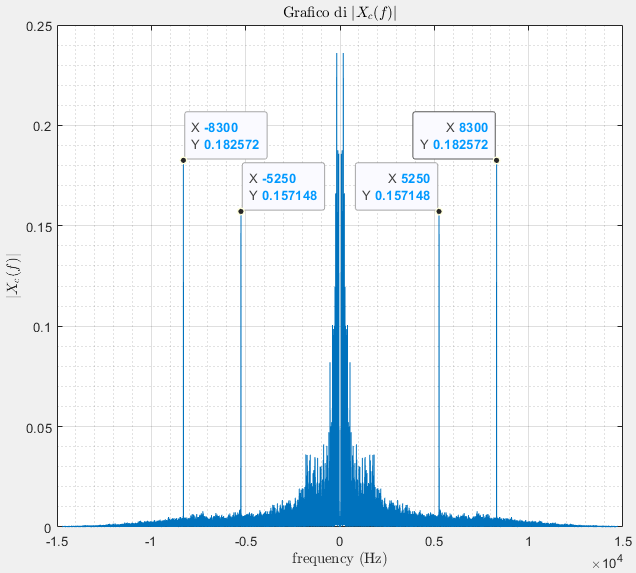
\includegraphics[width=0.5\linewidth]{./images/fft_x_c.png}
	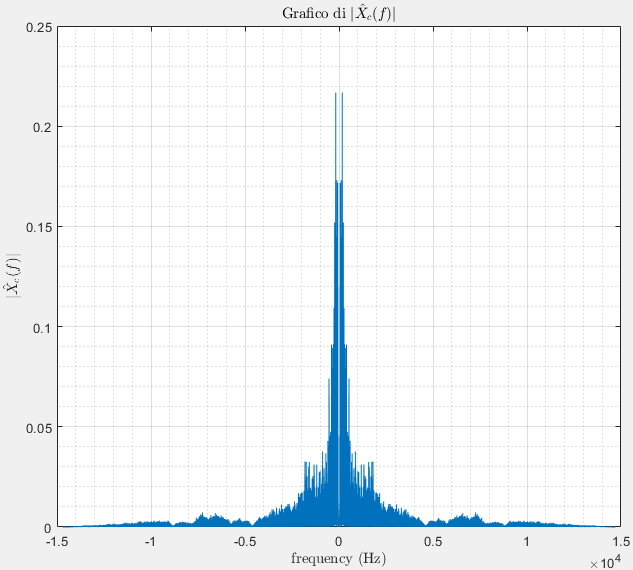
\includegraphics[width=0.5\linewidth]{./images/fft_x_c_hat.png}
\end{figure}

Dall'ascolto dei due segnali si nota come, oltre alla scomparsa dei due toni relativi alle componenti ad alta frequenza, nel secondo caso il segnale è più chiaro anche se leggermente più ovattato, soprattutto per alcuni toni (probabilmente per effetto dei notch filter). \hfill \break

Confrontando i grafici dei moduli delle trasformate dei due segnali $x_{c}$ e $\hat{x}_{c}$, si nota infatti la scomparsa dei picchi in $\pm5250Hz$ e $\pm8300Hz$ e la comparsa di alcuni avvallamenti, dovute all'intervento dei notch filter. 

\begin{figure}[H]
	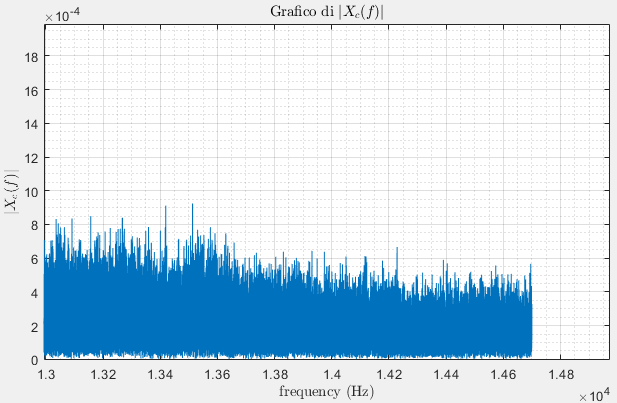
\includegraphics[width=0.5\linewidth]{./images/tail_fft_x_c.png}
	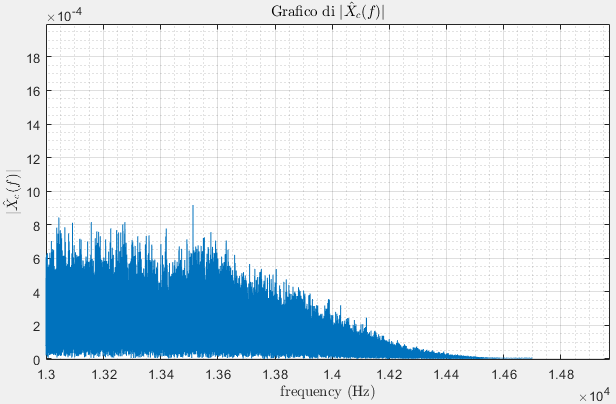
\includegraphics[width=0.5\linewidth]{./images/tail_fft_x_c_hat.png}
\end{figure}

Osservando in particolare le code in prossimità di $\pm\frac{F_{c}}{2}$, si può notare come in questa zona $|\hat{X}_{c}(f)|$ assuma valori generalmente minori rispetto a $|X_{c}(f)|$, per effetto dell'eliminazione della componente di aliasing e della attenuazione in banda provocata dal filtro passa-basso.

\end{document}
